\section{Results}

\subsection{Model Rankings and the Cross-Lingual Gap}


\begin{table*}[t]
\centering
\small
\setlength{\tabcolsep}{5pt}
\begin{tabular}{l ccc ccc ccc}
\toprule
 & \multicolumn{3}{c}{\textbf{Google Patents}} & \multicolumn{3}{c}{\textbf{EPO}} & \multicolumn{3}{c}{\textbf{Cross-lingual coverage}} \\
\cmidrule(lr){2-4}\cmidrule(lr){5-7}\cmidrule(lr){8-10}
Model & R@10 & CLIR & LT\% & R@10 & CLIR & LT\% & $k^\star_{80}$ & $k_{\mathrm{same}}$ & $k_{\mathrm{cross}}$ \\
\midrule
embeddinggemma            & \textbf{0.57} & \textbf{0.54} & 73          & \textbf{0.58} & \textbf{0.52} & 74          & \textbf{147}   & \textbf{36} & \textbf{121} \\
bge-m3                    & 0.51          & 0.47          & \textbf{74} & 0.55          & 0.47          & 66          & 304            & 66          & 215 \\
qwen3-0.6B                & 0.49          & 0.45          & 72          & 0.47          & 0.39          & 61          & 425            & 63          & 310 \\
nomic-v2-moe              & 0.46          & 0.41          & 63          & 0.51          & 0.43          & 63          & 367            & 55          & 321 \\
granite-278m              & 0.41          & 0.39          & 72          & 0.39          & 0.36          & 84          & $>$1000        & 641         & 569 \\
LaBSE                     & 0.30          & 0.27          & 59          & 0.27          & 0.25          & \textbf{85} & $>$1000        & 761         & $>$1000 \\
e5-large-instruct$^\dagger$ & 0.21        & 0.09          & 12          & 0.29          & 0.12          & 19          & $>$1000        & 47          & $>$1000 \\
SapBERT                   & 0.24          & 0.20          & 49          & 0.22          & 0.17          & 54          & $>$1000        & 807         & $>$1000 \\
\bottomrule
\end{tabular}
\caption{Retrieval performance on both patent offices. Best per column in bold.}
\label{tab:main-results}
\end{table*}

embeddinggemma leads on both offices and on every axis (Google Patents / EPO
Recall@10 0.57 / 0.58, CLIR@10 0.54 / 0.52) and reaches both golds the fastest
($k^\star_{80}{=}147$ vs.\ 304 for the next model), with bge-m3 a consistent second;
the ordering barely changes between the two offices, so it reflects the task ratherqwen3-0.6B and
nomic-v2-moe are mid-pack, while granite-278m, LaBSE and SapBERT trail by 20--30
Recall@10 points---and one model is an instructive outlier: e5-large-instruct looks
mid-pack on raw Recall@10 (0.21 / 0.29) but its CLIR@10 collapses to 0.09 / 0.12 and
its LT to 12 / 19, failing on cross lingual task. Off-the-shelf multilingual embedders are
therefore far from interchangeable on this task, and even the best absolute numbers
are low for an industrial deployment.


Across the whole field, retrieving a same-language copy of the answer is far easier
than retrieving its foreign twin and no model escapes the drop. The cross-lingual
coverage depths make the gap concrete: for the models that retrieve effectively the
same-language gold surfaces within a few dozen documents ($k_{\mathrm{same}}$
36--66) while its cross-language twin takes several hundred ($k_{\mathrm{cross}}$
121--321); for the weaker models both depths balloon and the cross-language gold is
frequently never covered for $80\%$ of queries within the retrieved top-1000. The
same pattern holds language by language: pooled across models, same-language recall
stays near 0.56--0.62 in every query language while cross-language recall sits around
0.34--0.38, a roughly 0.25 gap present in all five languages
(Figure~\ref{fig:home-advantage}); and the query$\times$document grid shows the loss lives off the diagonal for every
model (Figure~\ref{fig:qd-grid}): even the strongest retrievers fall to a fraction
of their same-language cell on individual routes, embeddinggemma drops from 0.69
same-language (English) to 0.18 when an English query must reach a German document,
bge-m3 from 0.62 (German) to 0.33 reaching a Spanish document, and nomic-v2-moe from
0.69 (French) to 0.12 reaching a Chinese one. Cross-linguality, not raw retrieval
power, is what every model struggles with.

\subsection{Alias-Graph: Inconsistency and Confusion}
\label{ssec:alias}

Asking the same compound in all five languages does not return the same patents.
The best cross-lingual RBO any model reaches is only 0.39 (embeddinggemma), a
ceiling no model beats (Figure~\ref{fig:alias}a), and it drops below 0.15 for the
weakest retrievers: two language variants of the same query share only a minority
of their top-ranked documents, so the embedding space is far from language-agnostic.


The second failure is chemical confusion: a wrong but chemically similar compound
out-ranks every gold patent on 14--48\% of queries depending on the model
(Figure~\ref{fig:alias}b, ALL column). The rate is strongly language-dependent, in
the direction the cross-lingual setting predicts. Averaged over models it is lowest
for English queries ($\approx$21\%) and highest for Chinese ($\approx$39\%), with
German, French, and Spanish in between ($\approx$28--30\%); the same chemical
question is markedly more likely to surface a look-alike above the right document
when it is asked in a lower-resource language than in English. The two failures
compound: a model that is both inconsistent across languages and easily confused by
near-neighbours is exactly the one a chemistry team must not deploy.

\begin{figure*}[t]
  \centering
  
\includegraphics[width=\linewidth]{claimD_D6_rbo_publication.png}
  \caption{Alias-graph failure modes across the eight models. \textbf{(a)}~Cross-lingual
  RBO: how much the top-ranked lists for the same compound asked in five languages
  overlap ($1=$ identical, $0=$ disjoint); the most consistent model reaches only
  $0.39$. \textbf{(b)}~Confusion rate: how often a chemically confusable look-alike
  out-ranks every gold patent, by query language and pooled (ALL column);
  $14$--$48\%$ overall, lowest for English and highest for Chinese.}
  \label{fig:alias}
\end{figure*}



\subsection{Reading Cost and the Re-Ranking Ceiling}
XRC asks a concrete operational question: starting from the top of the ranked list,
how much further must a user read to reach the foreign-language version of the answer
than to reach a same-language copy? Panel~(a) of Figure~\ref{fig:cost} reports the
median, and it is never one: the cheapest model still reads about twice as deep
(LaBSE, 1.9$\times$) and the rest three to six times deeper (bge-m3 3.5$\times$,
embeddinggemma 5.0$\times$, nomic-v2-moe 6.0$\times$). A low reading cost is not a
virtue on its own, though, the cheapest readers here are the weakest retrievers,
which read shallow only because they surface so little, so XRC has to be read together
with capability (CLIR@10), not minimized in isolation. We drop e5-large-instruct from
all three panels because it fails the CLIR@10 $<0.10$ degeneracy gate: it almost never
retrieves a foreign twin at all, so its reading-depth ratio explodes (median
161$\times$) and its recoverability curve rests on mostly censored ranks, the
instruments are undefined for a model that does not retrieve the thing whose depth
they measure.


The other two panels ask what a downstream re-ranker could do about the buried
cross-language documents. A re-ranker only reorders the candidate pool it is handed,
so RRC@$K$ (panel~b) the fraction of cross-lingual queries whose first cross-language
gold (the answer's document in another language) has appeared by rank $K$, is a hard
ceiling on what re-ranking can recover: anything past depth $K$ is invisible to a
top-$K$ re-ranker. Two things stand out. First, the recoverable documents are
front-loaded: the knee $K^\star$, the point of sharpest diminishing returns on the
curve, sits at $2$--$5$ for the strong models, so a shallow top-5 pool already captures
the bulk of the cheaply recoverable cross-language gold (embeddinggemma RRC@5 $=0.53$);
a deeper pool keeps helping but with falling efficiency per decade (RRC@100 $=0.78$,
RRC@1000 $=0.93$), while the weak LaBSE and SapBERT reach their knee only at depth
$75$--$150$. Second, even an exhaustive re-ranker over the full retrieved pool hits a
wall: panel~(c) splits each model's cross-lingual shortfall into what a cheap top-10
re-rank recovers, what a deeper pool up to top-1000 adds, and an alignment-only floor
beyond the top-1000, cross-language gold that first-stage retrieval never surfaces and
that no re-ranker over the retrieved candidates can reach. That floor is $7\%$ of the
gap for embeddinggemma and grows to $27\%$ for SapBERT: the weaker the model, the more
of its cross-lingual failure is structural. And a realistic top-100 re-ranker recovers
even less, bounded by RRC@100 ($0.78$ for the best model), it reorders only what
first-stage retrieval already placed in its pool, so the durable fix for the residual
gap is representation alignment at indexing time, not a re-ranker at query time.



\begin{figure*}[t]
  \centering
  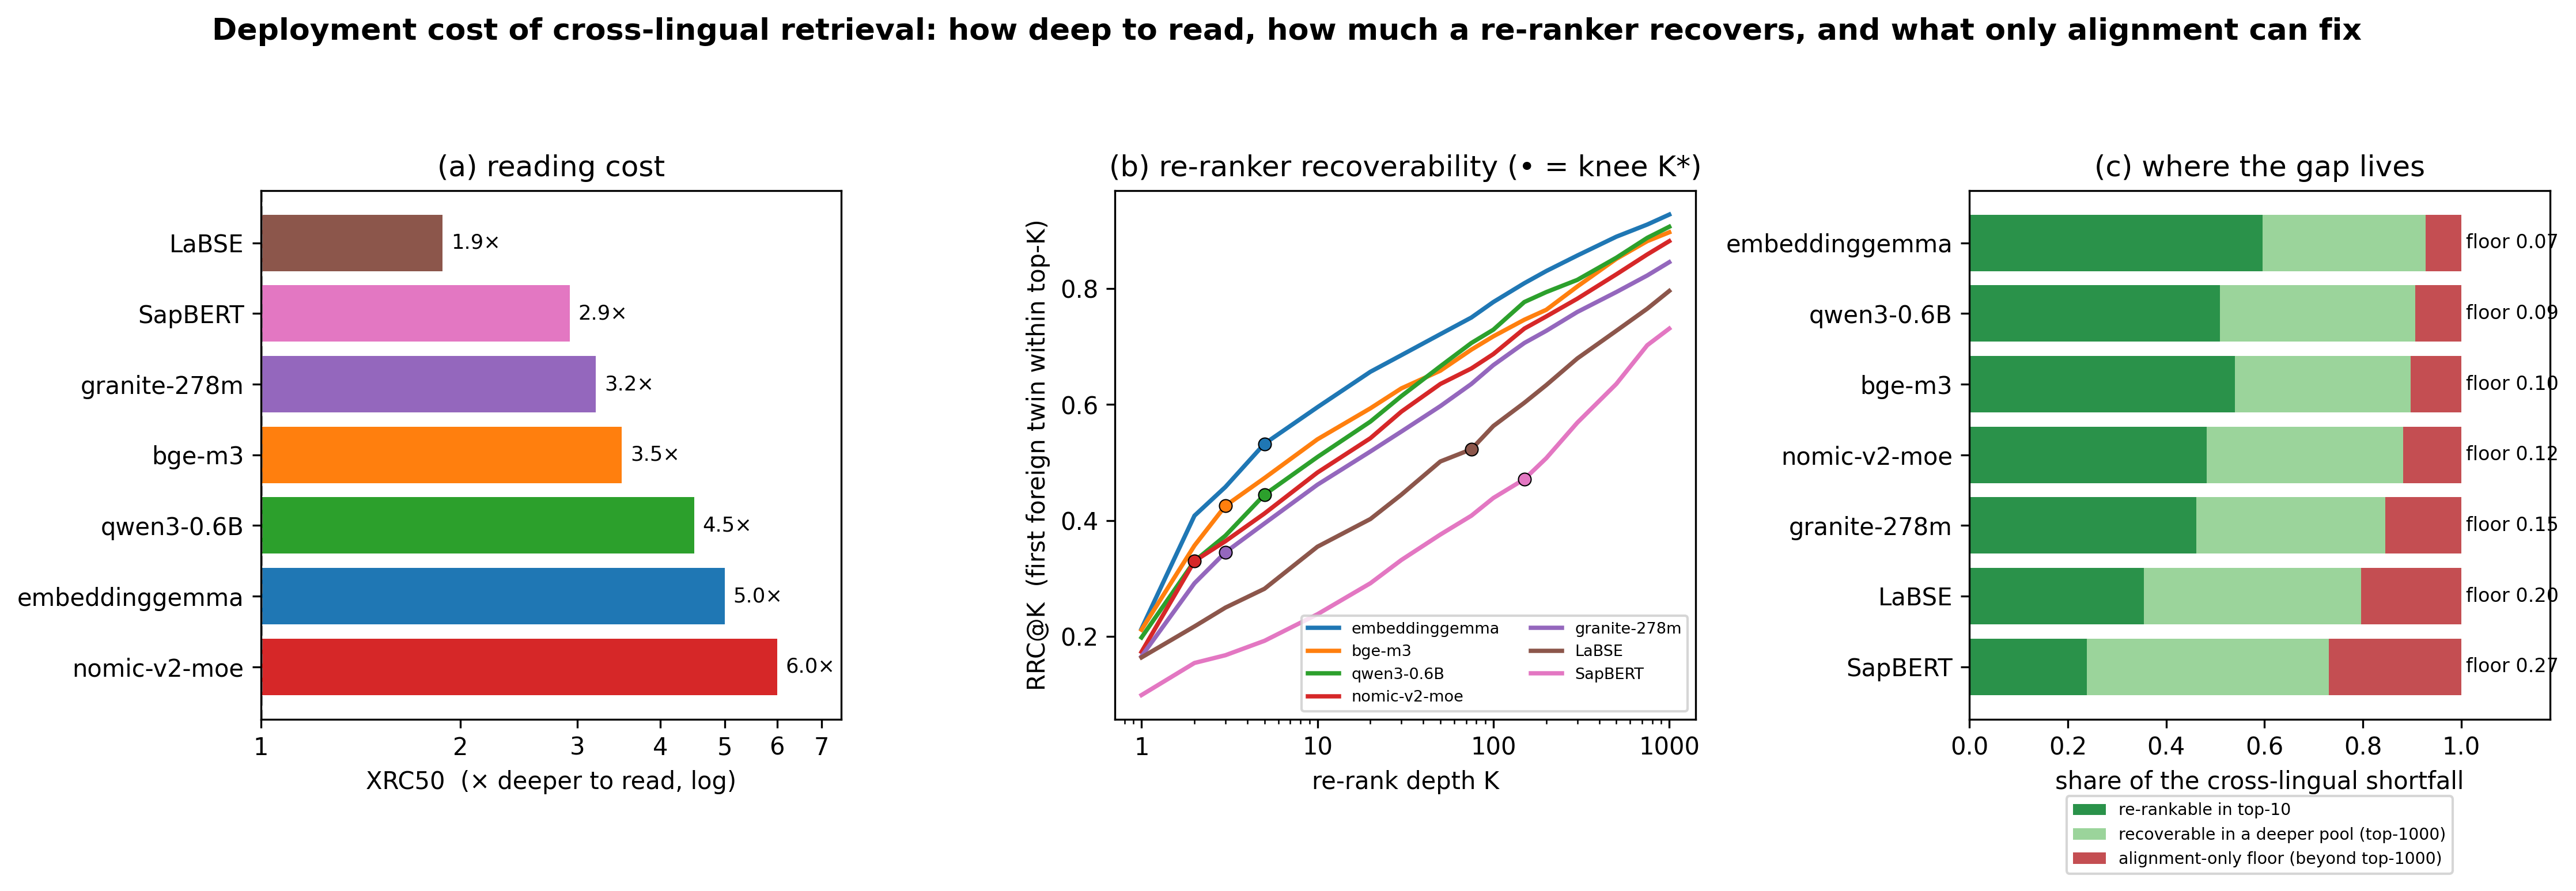
\includegraphics[width=\linewidth]{figures/claimE_E2_triptych.png}
  \caption{Deployment cost of cross-lingual retrieval (e5-large-instruct excluded by
  the CLIR@10 $<0.10$ gate). \textbf{(a)}~XRC50 reading cost; \textbf{(b)}~RRC@$K$
  re-ranker recoverability with knee $K^\star$ ($\bullet$); \textbf{(c)}~the shortfall
  split into re-rankable (top-10), deeper-pool (top-1000), and an alignment-only floor.}
  \label{fig:cost}
\end{figure*}
